\documentclass[a4paper]{article}

\usepackage[english]{babel}
\usepackage[utf8]{inputenc}
\usepackage{amsmath}
\usepackage{graphicx}
\usepackage[colorinlistoftodos]{todonotes}
\usepackage{float}

\title{Usability of iTunes and Spotify}

\author{Matthew Flickner}

\date{\today}

\begin{document}
\maketitle

\begin{abstract}
In CMSI 370, Interaction Design, we have been studying usability measurements and assessing how well software complies with its guidelines as well as design principles, and theories. Our group decided to test Music Applications. After a short discussion we decided that iTunes and Spotify were the two current titans clashing for user dominance. Through our field testing and analysis we discovered that Spotify better implements design principles and theories, making it more efficient to use and better able to satisfy users than its rival iTunes.
% JD: The causality statement in the last sentence should be reversed---you first found
%     that Spotify had better metrics, and then based on analysis you noticed a correlation
%     between guideline/principle/theory compliance and this performance.
\end{abstract}

\begin{figure}[H]
\centering

\includegraphics[width=0.2\textwidth]{ITunes_11_Logo.png}

\includegraphics[width=0.2\textwidth]{spotifylogo.jpg}
\end{figure}

\section{Introduction}

Music software for years has, for the most part, been dominated by Apple through iTunes. iTunes was always the simplest and easiest to use. There were others such as Windows Media Player and Rhapsody that tried to rival iTunes but none really could. So iTunes reigned supreme. But now a new challenger, Spotify has entered the game. Its popularity has risen mostly through the fact that it does not require users to actually buy songs to be able to listen to them in full. Rather a free subscription gives unlimited access to any song the user desires with ads in between every few songs and paying for a monthly subscription removes the ads. But features mean nothing if the software is not user-friendly.
% JD: Despite these two products' being pretty well-known, in formal written work it would
%     still be appropriate to cite even just their websites.

\section{Usability Metrics}
\label{sec:usabilityMetrics}

\subsection{The Field Test}
Our team decided to perform field tests to measure the Usability Metrics in Spotify and iTunes. Before each user performed the test, their level of experience with the software was recorded. Ideally we would have liked to be able to test \textit{Learnability} but our subject pool on the iTunes side were all familiar with iTunes which gave us no grounds for comparison with test subjects who had never used Spotify before. So instead, we will evaluate iTunes and Spotify for \textit{Efficiency}, \textit{Errors}, and \textit{Satisfaction}.

\subsection{The Users}
Before diving into the field test, some background information on the users is necessary to be able to better understand and interpret the data.
\begin{figure}[H]
\centering
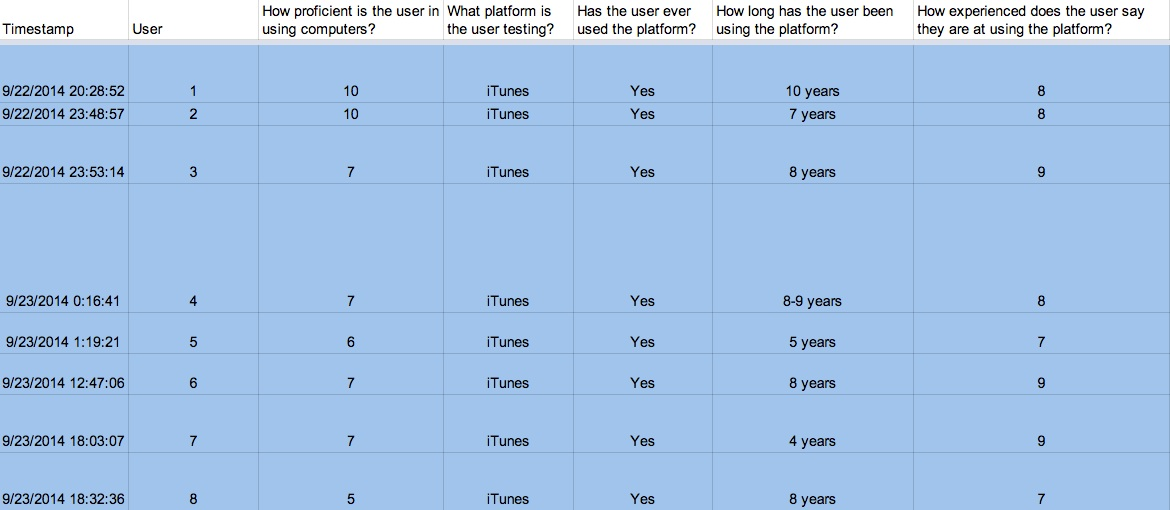
\includegraphics[width=1\textwidth]{itunesuserbackground_copy.jpg}
\caption{\label{userdata: itunes}iTunes User Background}
\end{figure}
\begin{figure}[H]
\centering
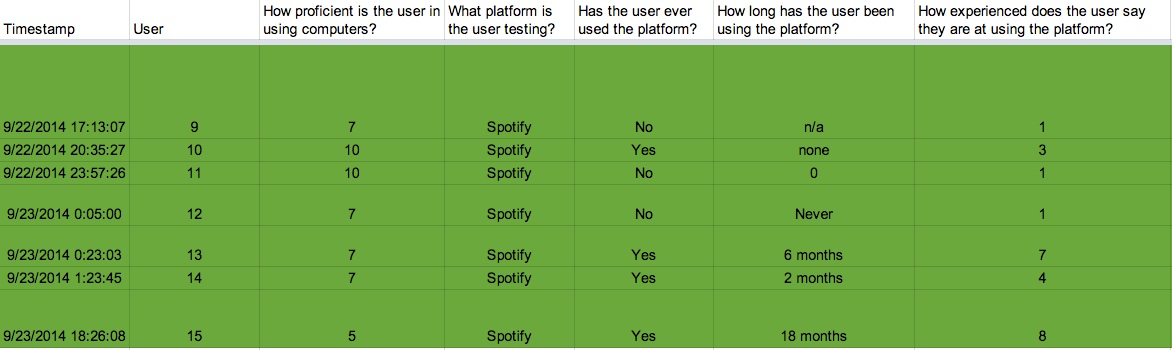
\includegraphics[width=1\textwidth]{spotifyuserbackground_copy.jpg}
\caption{\label{userdata: spotify}Spotify User Background}
\end{figure}
iTunes users rated their proficiency with computers at an average of 7.375 and Spotify users rated their computer proficiency at 7.5714 so both groups are very similiar with overall computer proficiency. Spotify users had an average experience level of only 3.57 with using Spotify. iTunes users reported an average experience level 8.125 with iTunes, suggesting they are far more familiar with the iTunes software than the Spotify users were with Spotify. 
% JD: Although this rating, typically called "self-efficacy," can be useful in certain
%     studies, for this one, its main indication is to point at a chronological gap
%     between iTunes and Spotify users.  The best course of action after this finding
%     is to allow all subjects to use both applications for some extended "free time,"
%     in order to build up proficiency.  This ensures that what you're measuring later
%     is truly efficiency, and not some potential combination of learnability and
%     efficiency mixed in.
%
%     (and yes, even with the eventual results, this adjustment is a good thing to do)

\subsection{The Tasks}
Each user was asked to perform the following tasks. Users were timed and their satisfaction evaluated on a scale of 1 to 10. Any errors the users made were documented by the proctor of the test.
\begin{enumerate}
\item Starting out on the music library of the platform, time how long it takes the user to create a new playlist with the title ``Hello World.''
\item Starting out on the music library of the platform, record how long it takes for the user to start ``Tiesto Radio.''
\item Start out on the main music library of the app. Record how long it takes the user to go to the existing playlist and set the playlist to repeat indefinitely.
\end{enumerate}

\subsection{The Results}
  \begin{itemize}
      \item \textbf{Task 1:}
      
          \begin{figure}[H]
              \centering
              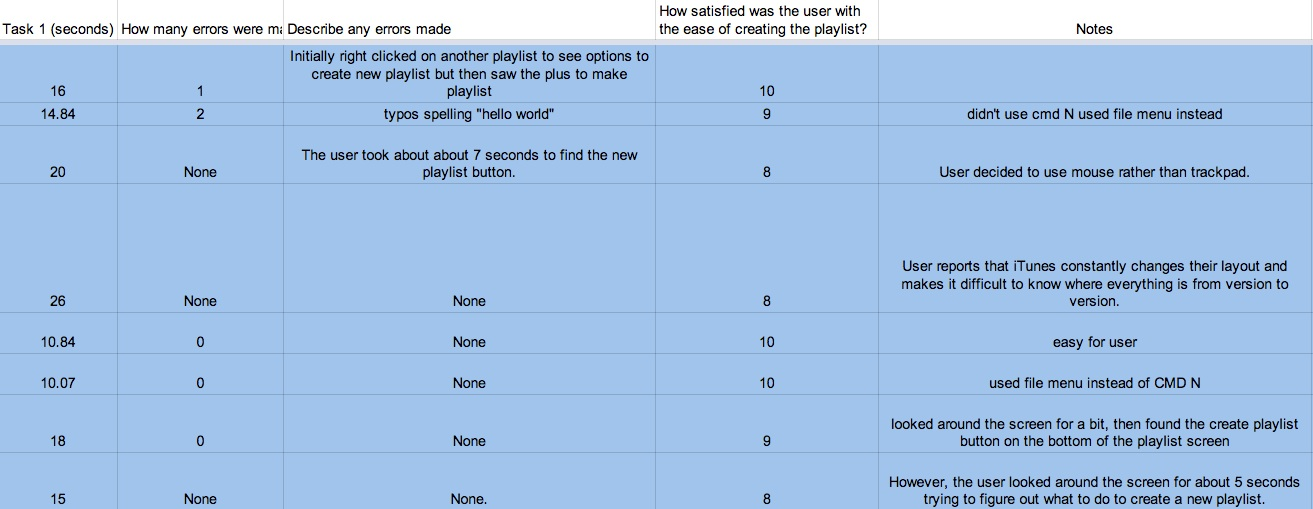
\includegraphics[width=1\textwidth]{itunestask1_copy.jpg}
              \caption{\label{tasks: task1itunes}iTunes Results 1}
          \end{figure}
          \begin{figure}[H]
              \centering
              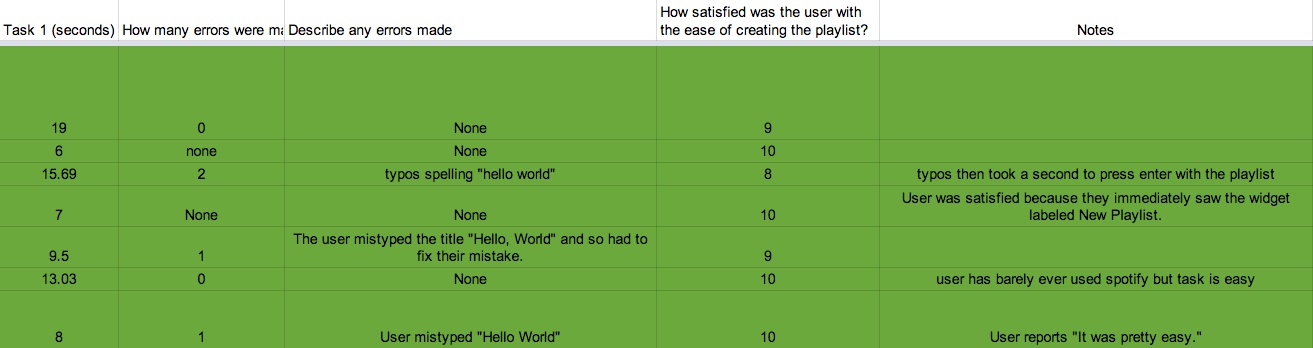
\includegraphics[width=1\textwidth]{spotifytask1_copy.jpg}
              \caption{\label{tasks: task1spotify}Spotify Results 1}
          \end{figure}
    
      The average time it took users on iTunes to perform Task 1 was 16.34 seconds while the average time on Spotify was 11.17 seconds. As far as errors go all errors on Spotify were user typos spelling the playlist name ``Hello World'' which is not even an error involving confusion on how to use Spotify rather user input error. There were few errors in iTunes but they involved trying to find how to create a new playlist. As far as satisfaction goes, for Task 1, iTunes had an average satisfaction rating of 9 and Spotify had a 9.42 satisfaction rating. Users on iTunes often did not see the create playlist button and instead went into the file menu to create a playist while Spotify users saw the widget to create a playlist immediately.\\
    
      \item \textbf{Task 2:}
      
          \begin{figure}[H]
              \centering
              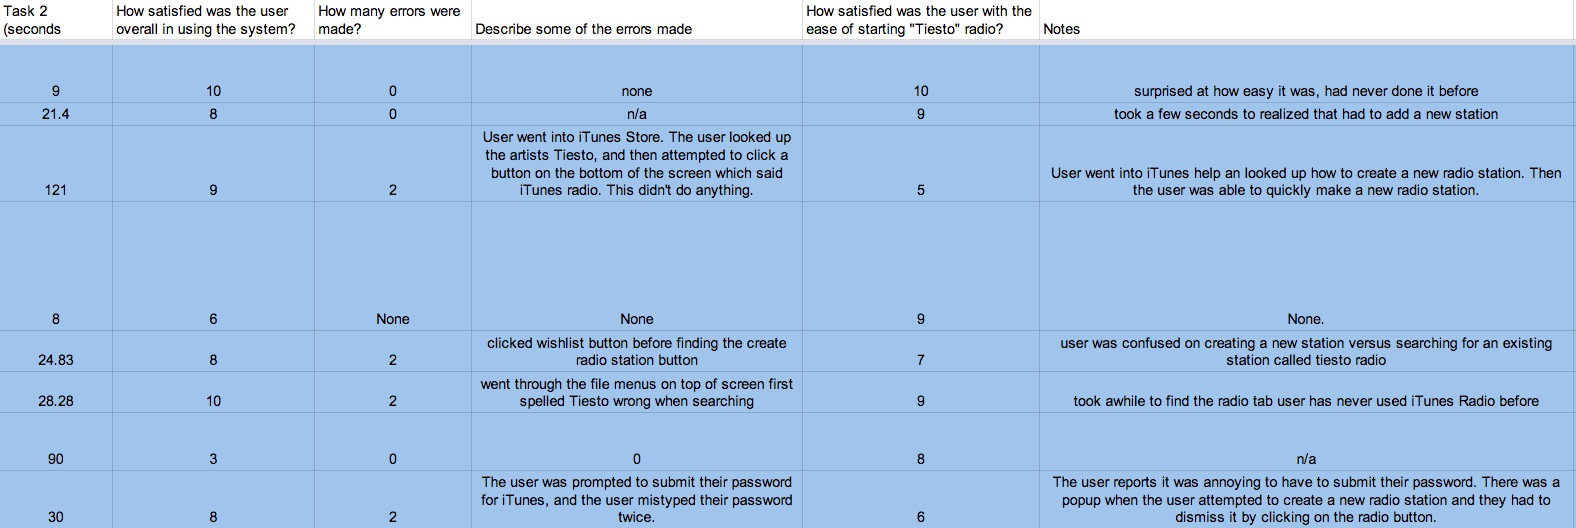
\includegraphics[width=1\textwidth]{itunestask2_copy.jpg}
              \caption{\label{tasks: task2itunes}iTunes Results 2}
          \end{figure}
          \begin{figure}[H]
              \centering
              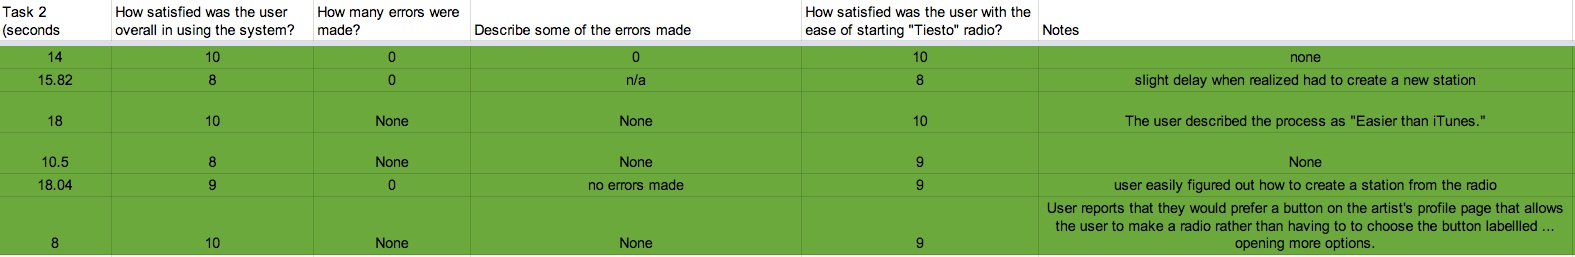
\includegraphics[width=1\textwidth]{spotifytask2_copy.jpg}
              \caption{\label{tasks: task2spotify}Spotify Results 2}
          \end{figure}
          
      The average time it took users on iTunes to complete Task 2 was 41.56 seconds while Spotify users took an average of 20.62. It should be noted that iTunes had more extreme outliers than Spotify but the experienced iTunes users were still clearly a good deal slower than the newer Spotify users. The average satisfaction of iTunes users was 7.88 while the Spotify users average was a score of 8, still beating iTunes despite the fact that one Spotify user gave it a score of 1. iTunes had 4 user errors made while Spotify only had one user make an error.  \\
      
      
      \item \textbf{Task 3:}
     
          \begin{figure}[H]
              \centering       
              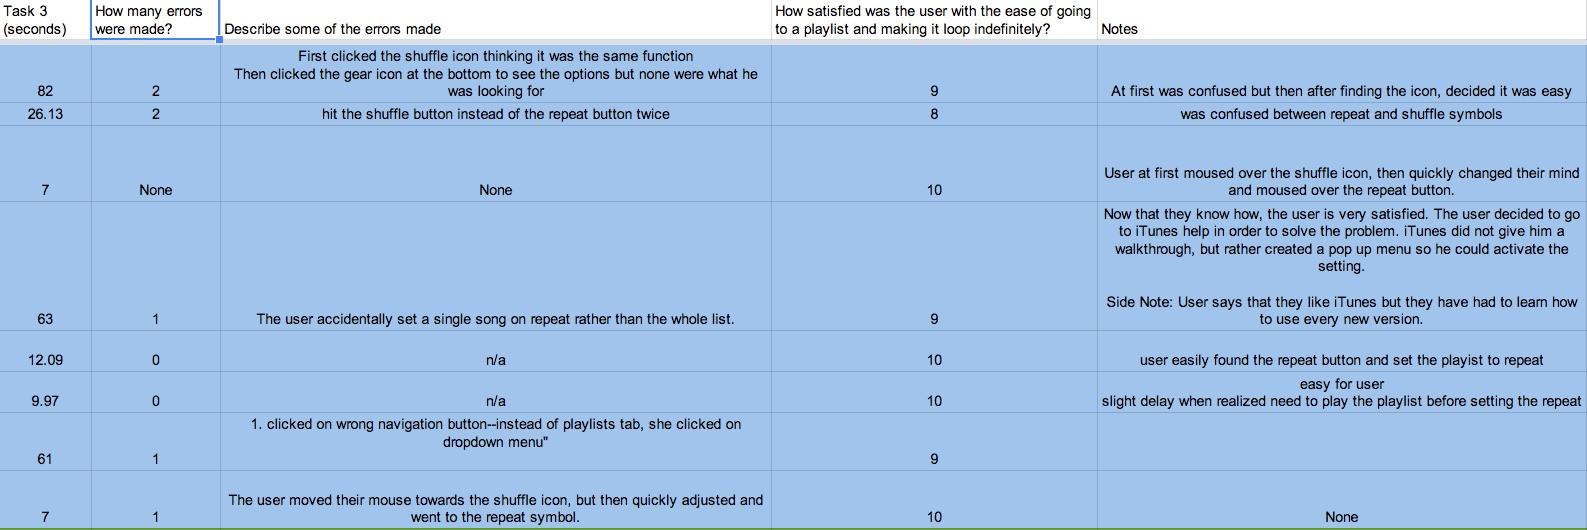
\includegraphics[width=1\textwidth]{itunestask3_copy.jpg}
              \caption{\label{tasks: task3itunes}iTunes Results 3}
          \end{figure}
          \begin{figure}[H]         
              \centering
              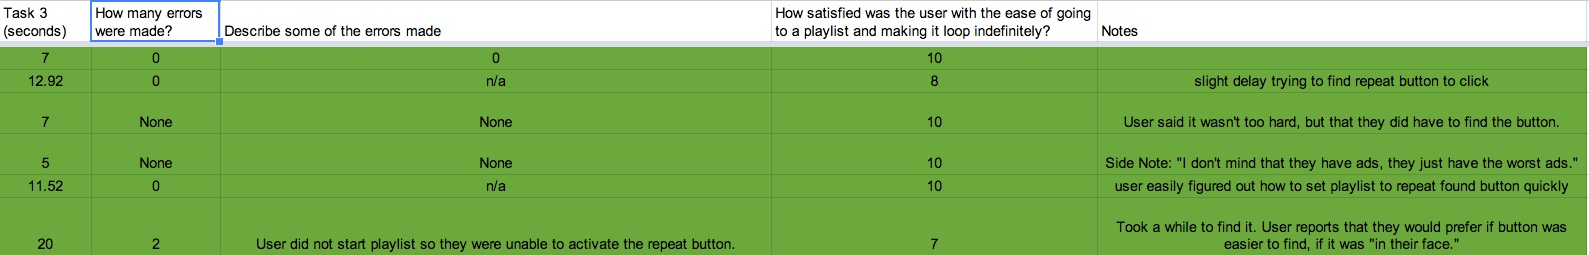
\includegraphics[width=1\textwidth]{spotifytask3_copy.jpg}
              \caption{\label{tasks: task3spotify}Spotify Results 3}
          \end{figure}
          
          On average it took iTunes users 33.52 seconds to complete Task 3. This is suprisingly high considering their experience. Spotify users took on average 20.06 seconds. Both groups had an outlier of over 60 seconds. iTunes users made 7 errors opposed to Spotify's 4 errors. A common error in iTunes was users going for the shuffle button instead of mousing to the repeat button. As far as satisfaction goes iTunes users  rated their satisfaction at a average of 9.375 while Spotify users rated at an average of 8.71, a bit lower than iTunes.
      
  \end{itemize}
  
\subsection{Overall Efficiency}
There is no doubt that Spotify is the winner of the efficiency battle. Spotify demolished iTunes in average time elasped to complete each task despite the fact that users had far less experience with using Spotify.
\begin{figure}[H]
\centering
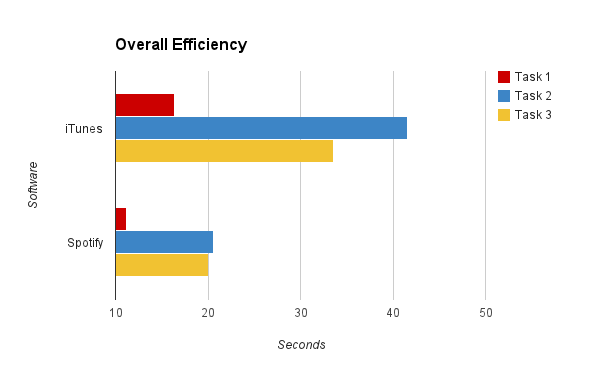
\includegraphics[width=0.6\textwidth]{efficiencyoverall.png}
\caption{\label{overall: efficiency} Overall Efficiency}
\end{figure}

\subsection{Overall Errors}
With regards to errors, iTunes totaled 18 errors. Spotify only had 10 user errors. Most errors involved either a typo or the user being unable to locate where the button to perform a certain function was located. Users of Spotify experienced significantly less errors.

\subsection{Overall Satisfaction}
  At the end of the day, after the users had finished the tasks and the usability tests, they ranked their overall satisfaction. iTunes had an average satisfaction was a 7.75 while Spotify's average satisfaction was a 9. Despite not being nearly as experienced as the iTunes users, the Spotify users were far more satisfied than the users of iTunes.
\begin{figure}[H]
\centering
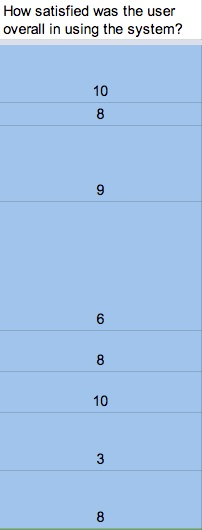
\includegraphics[width=0.15\textwidth]{itunes_satis.jpg}
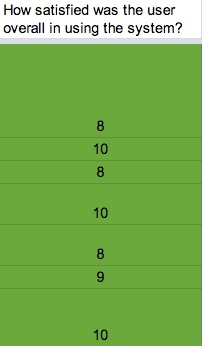
\includegraphics[width=0.15\textwidth]{spotifysatis__copy.jpg}
\caption{\label{overall: satisfactionSpotify} iTunes (Blue) vs Spotify (Green) Satisfaction}
% JD: Watch the layout of this figure---from afar, it can be misinterpreted as a bar
%     graph with iTunes looking higher!
\end{figure}


\section{Heuristic Evaluation}
\label{sec:heuristicEval}
The data definitely speaks for itself. Spotify clearly dominated iTunes in every aspect. Spotify users were more efficient, more satisfied, made less errors despite less experience. Both Spotify and iTunes have done good things with their software but Spotify has cleary implemented a few sublte design principles and theories better than iTunes. Since efficiency leads very often to fewer errors and higher satisfaction, we will analyze the efficiency side of our field tests to see what Spotify did to make their software more efficient than iTunes.

\subsection{Head to Head: Creating a New Playlist}
In Spotify, the ``New Playlist'' button is clearly visible in the left side menu. But what mades Spotify really excel is its implementation of Fitts's Law. Upon clicking the ``New Playlist'' button, the new playlist appears right below it, ready to be named thus minimizing the distance a user must travel in order to name the playlist.
% JD: Nice observation.
\begin{figure}[H]
\centering
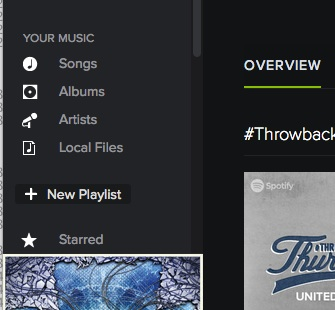
\includegraphics[width=.3\textwidth]{spotifyplaylist1_copy.jpg}
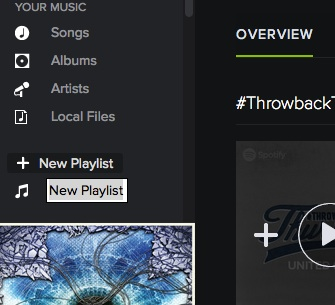
\includegraphics[width=.3\textwidth]{spotifyplaylist2_copy.jpg}
\caption{\label{heuristic: playlistSpotify} Creating a New Playlist in Spotify}
\end{figure}
On the other hand iTunes fails to implement this as efficiently. In iTunes, everything depends on which menu on the top of the window the user has selected. If anything other than ``Playlists'' is selected in the top menu, then the only way to create a new playlist by going into the file menu the the very top of the screen. If the ``Playlists'' is selected then the user can mouse down to the bottom-left of the window and then click on the small plus sign there. They then must select what kind of playlist they wish to create.

\begin{figure}[H]
\centering
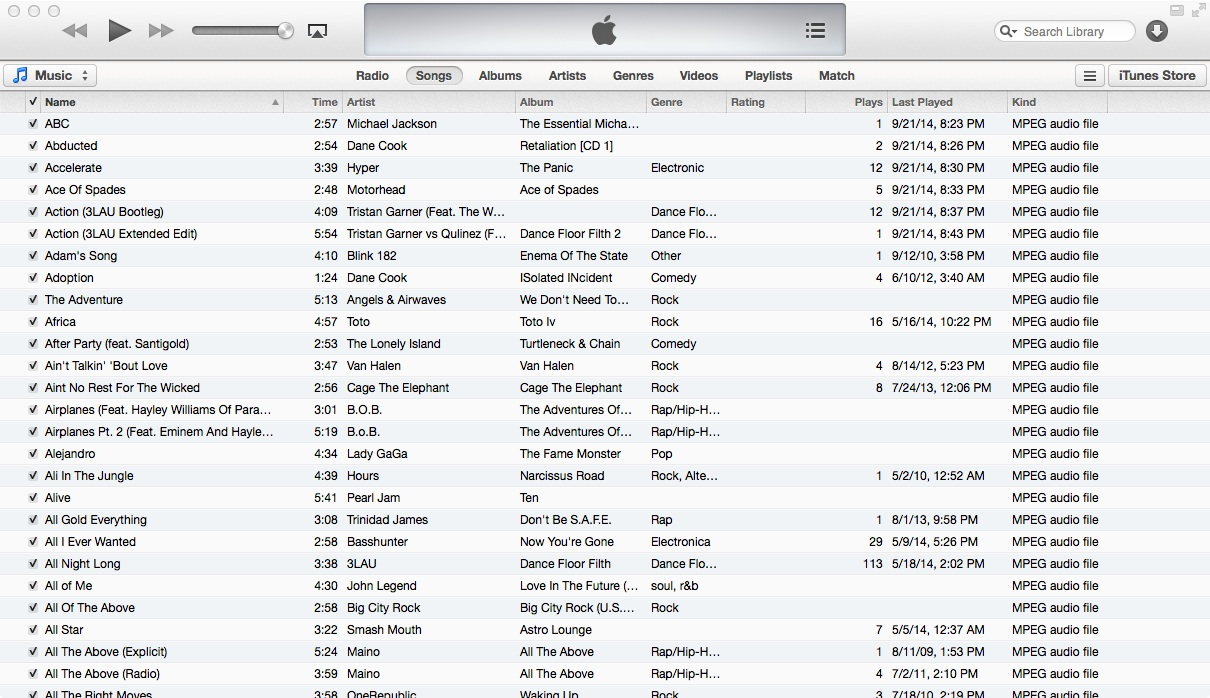
\includegraphics[width=.6\textwidth]{itunesfromsongs.jpg}
\caption{\label{heuristic: iTunesSongs} iTunes from Songs}
\end{figure}
\begin{figure}[H]
\centering
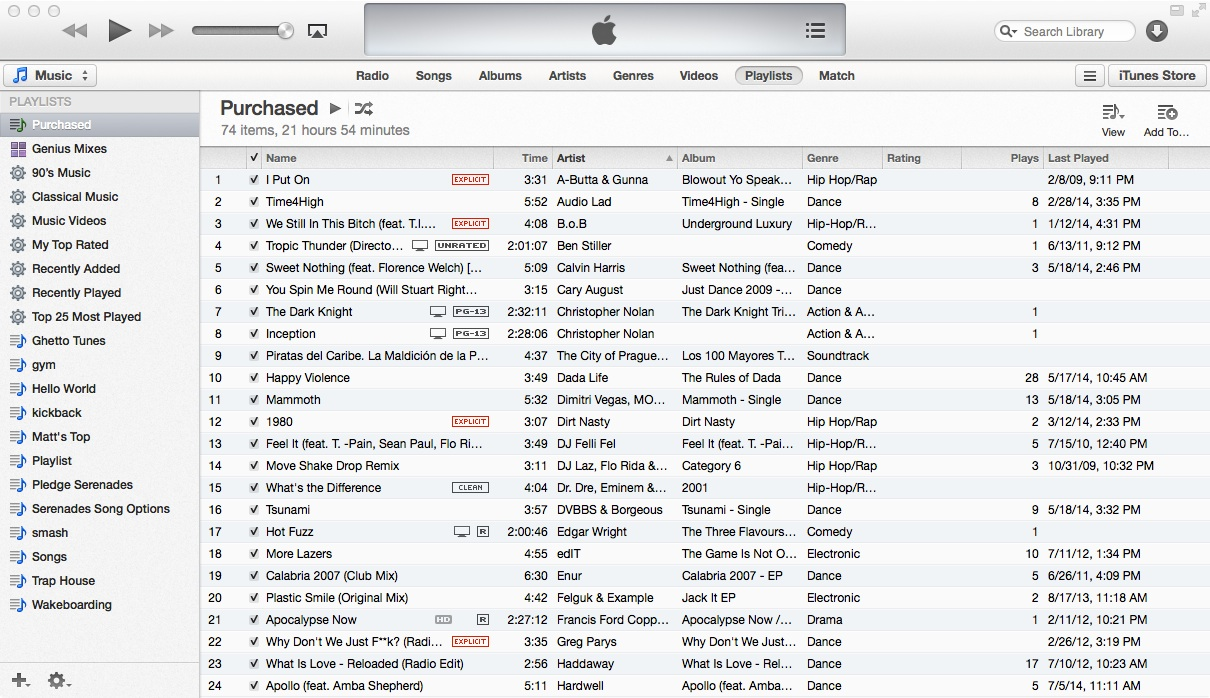
\includegraphics[width=.6\textwidth]{itunesfromplaylists.jpg}
\caption{\label{heuristic: iTunesPlaylists} iTunes from Playlists}
\end{figure}

Upon creating a playlist, the iTunes user must focus their attention to the other side of the window, on the top-right. This is were a side window on the right pops up and allows them to name their new playlist.

\begin{figure}[H]
\centering
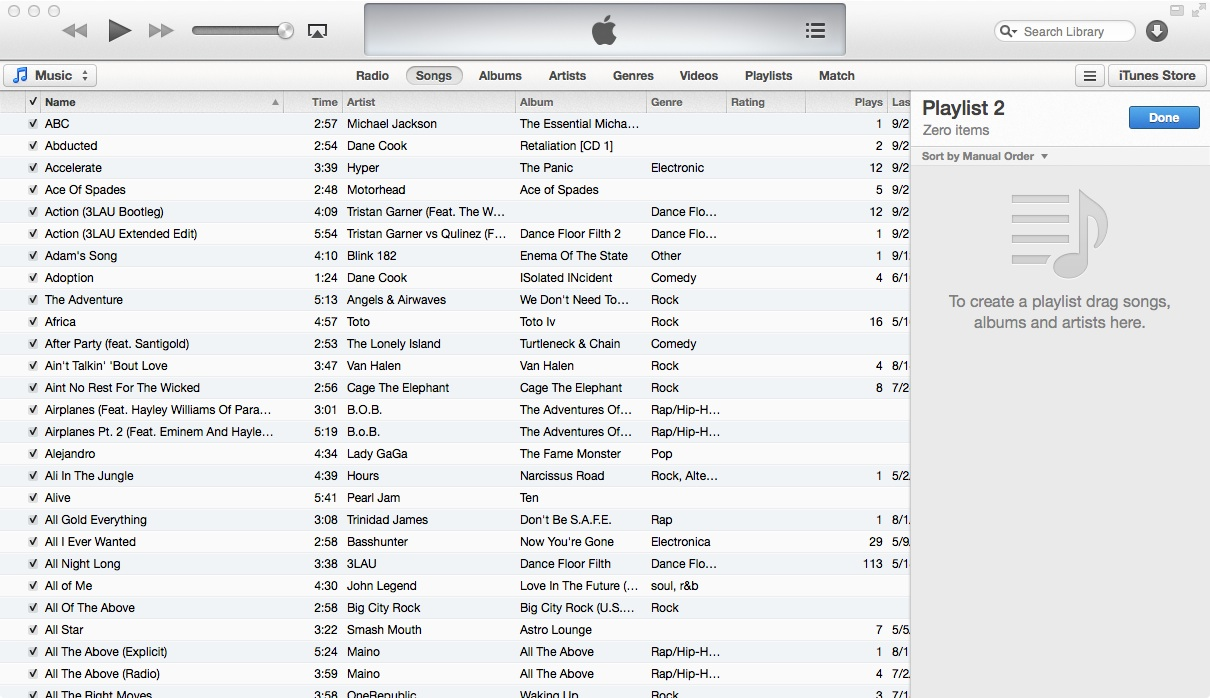
\includegraphics[width=.6\textwidth]{itunescreateplaylist.jpg}
\caption{\label{heuristic: iTunesPlaylistCreate} Creating a New Playlist in iTunes}
\end{figure}

iTunes deserves some credit for at least working on a diagonal line across the window but the amount of distance traveled and the number of steps it takes to make a playlist on iTunes is the reason iTunes lost to Spotify in the efficiency battle.

\subsection{Head to Head: Using the Radio Feature}
The Radio feature is a new one in most music applications and as the data shows Spotify users were once again far more efficient completing this task than iTunes users. In this case, the issue came down to modality and more specifically, dialogue layout. Both iTunes and Spotify utilize proper top-left to bottom-right sequencing but Spotify has utilized it in a far more efficient way.
% JD: Where did you derive the guideline that top-left-to-bottom-right is a recommended
%     arrangement for information?
In iTunes, to get to Radio, the user must click on the Radio button in the top menu. Once in Radio, the user must get all the way down to the bottom of the window in order to get to the "Create A Station" button.

\begin{figure}[H]
\centering
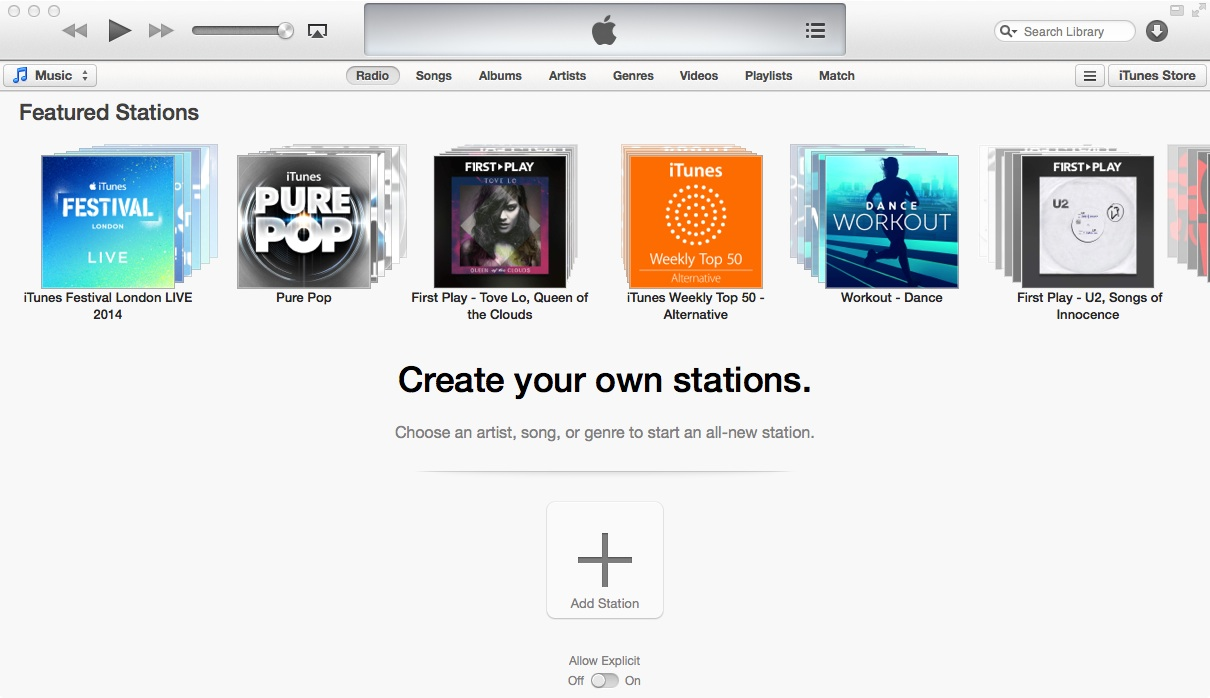
\includegraphics[width=.6\textwidth]{itunesradio.jpg}
\caption{\label{heuristic: iTunesRadio} Creating an iTunes Radio Station}
\end{figure}

Upon entering opening Radio in iTunes, the user's attention is on the Radio button in the top menu that they just clicked. They begin to move down and the first things their eyes catch is the Featured Stations and the line of colorful albums laid out horizontally across the window. The user naturally will move from left to right then down looking for the create a station button. iTunes clearly wants to get the user focused on the featured stations first before creating their own station.\\

On the other hand, Spotify's left to right dialogue layout is more focused on the user having their unique experience. Spotify radio can be accessed from the top of its left-hand menu.

\begin{figure}[H]
\centering
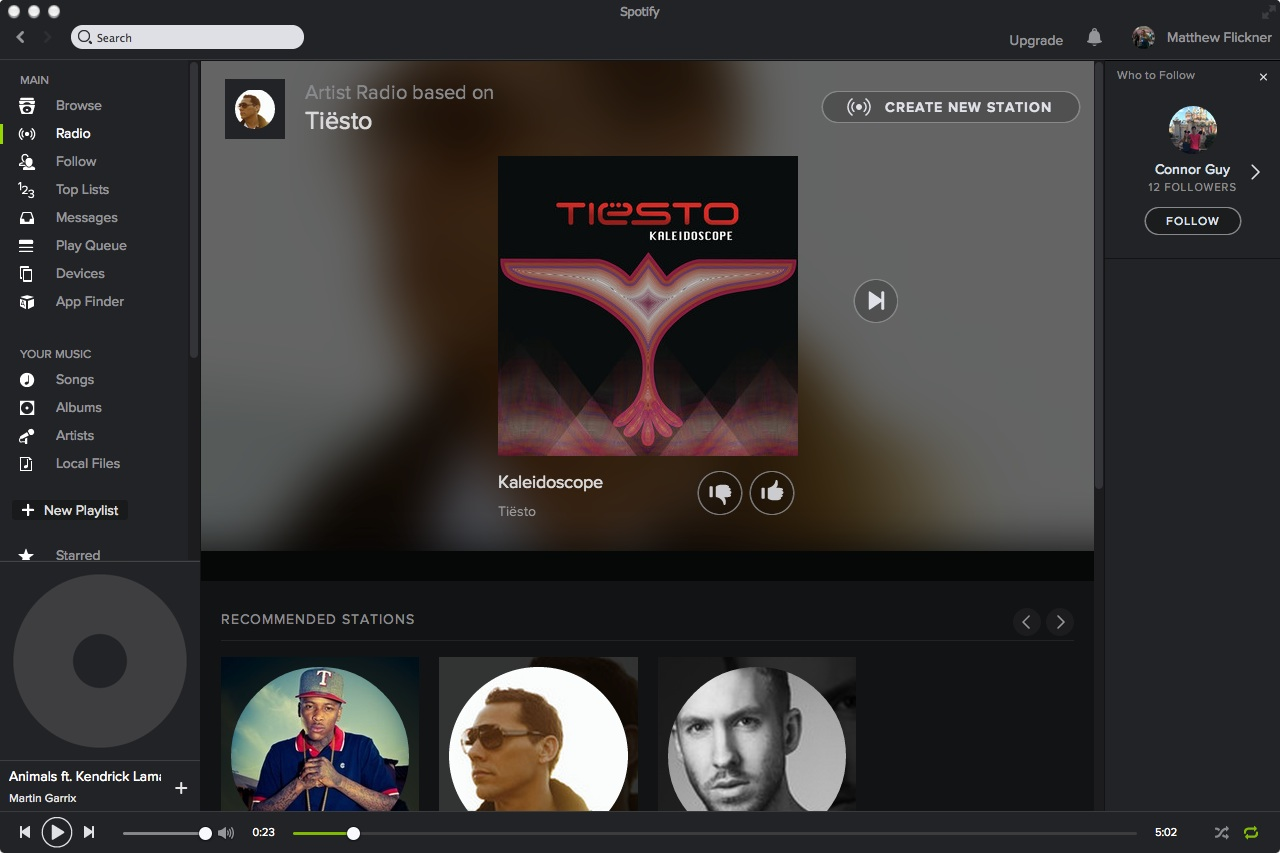
\includegraphics[width=.6\textwidth]{spotifyradio.jpg}
\caption{\label{heuristic: spotifyRadio} Spoitfy Radio}
\end{figure}

First thing in the top left is a recommendation based off the user's existing stations. From their moving right is the "Create New Station" button. Then below that is one album picture. The user then actually must scroll down to get to all other aspects of Spotify Radio. This minimizes user distraction for creating a station. An added aspect of Spotify's efficiency is more solid implementation of Fitt's Law. When the ``Create New Station'' button is clicked, the menu for a new station appears literally right on top of the button and thus on top of where the mouse is and the user's attention is.

\begin{figure}[H]
\centering
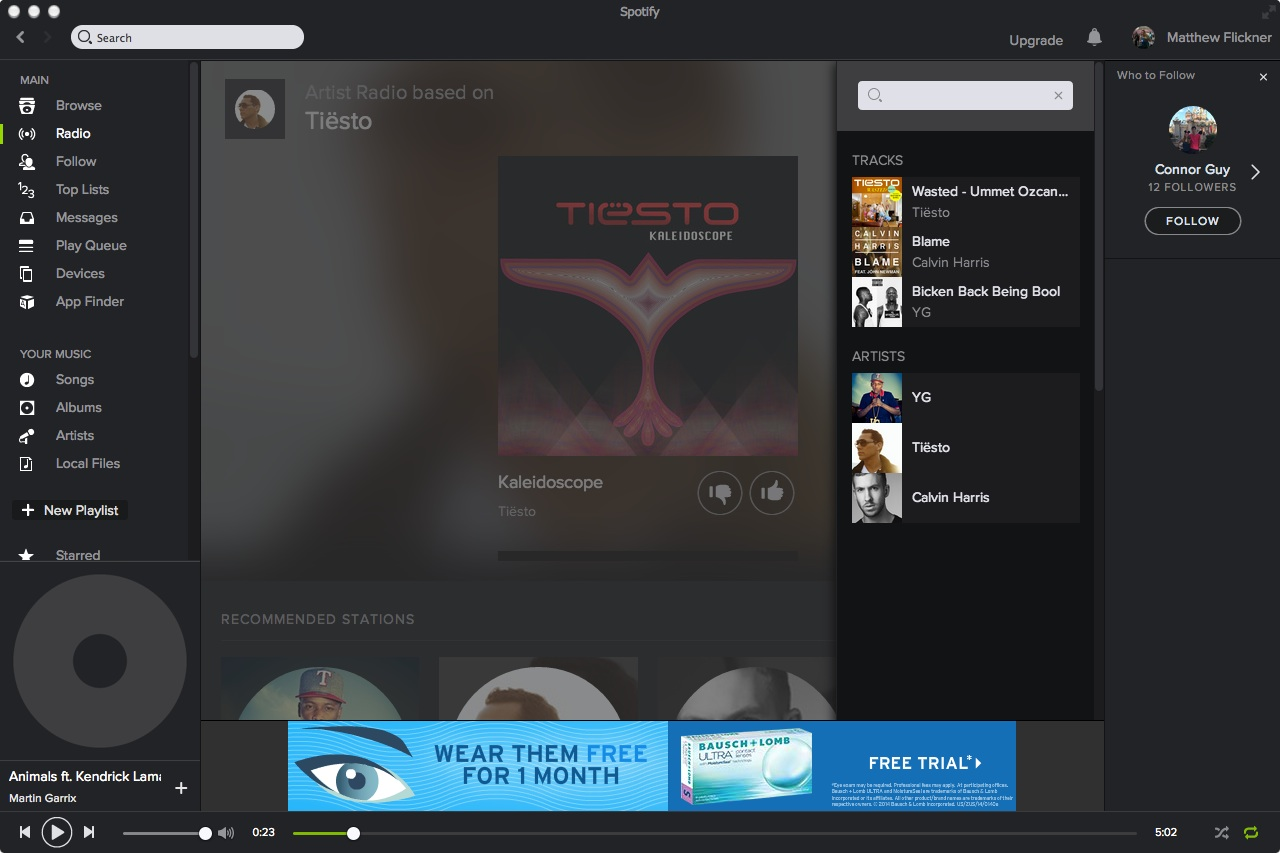
\includegraphics[width=.6\textwidth]{spotifyradio2.jpg}
\caption{\label{heuristic: spotifyRadio2} Creating a New Spotify Radio Station}
\end{figure}

In addition Spotify blurs the background, which prevents errors by direct manipulation. Spotify immediately drawing even more focus and clarity to the creating of the radio station. In contrast, the iTunes menu appears slightly above and to the right of the button. A slight difference in positioning but a huge one in maximizing user efficiency. 

\subsection{Head to Head: Repeating a Playlist}
Repeating a playlist was by far the most interesting of the results. Despite being more efficient, this is the one task that iTunes users were more satisfied despite being slower at completion. In additions iTunes users were more satisfied even though they made more errors. The errors in iTunes stemmed from one thing more than anything. iTunes users became confused with the larger shuffle icon next to the playlist name and the actually repeat button in the bottom-left of the miniplayer at the top of the window. 

\begin{figure}[H]
\centering
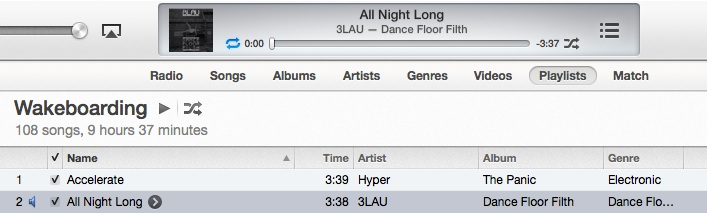
\includegraphics[width=.6\textwidth]{itunesrepeat.jpg}
\caption{\label{heuristic: iTunesRepeat} iTunes Repeat Button (blue)}
\end{figure}

However once users realized their error and found the actual repeat button they were more frustrated with themselves for not realizing something so simply than frustrated with iTunes. However the principle of the matter is that the larger shuffle icon drew their attention first.\\

With Spotify, the icons are the same size but they are located in the very bottom-right of the window.

\begin{figure}[H]
\centering
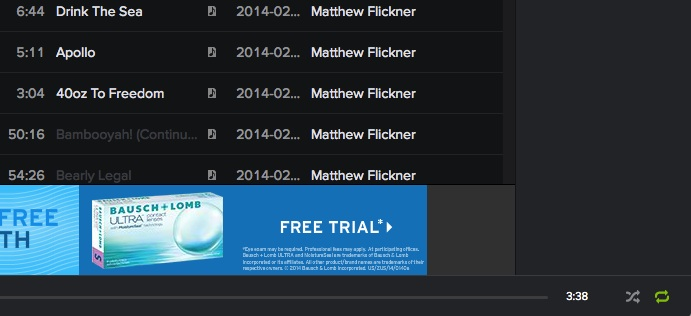
\includegraphics[width=.6\textwidth]{spotifyrepeat.jpg}
\caption{\label{heuristic: SpotifyRepeat} Spotify Repeat Button (Bottom Right)}
\end{figure}

Spotify users reported that they had to really look for it and wished it was more in their face. This has a lot to do with dialog layout, with something in the bottom-right of the window being naturally the last thing a user scans for.
% JD: ...for users whose language reads left-to-right, top-to-bottom :)

\section{Conclusion}
iTunes clearly lost this battle to Spotify for a few very good reasons. Spotify implemented Fitt's law far more effectively than iTunes did with it by minimizing distance users had to travel across the screen. In addition, Spotify focused on dialogue layout to make sure it was clear and fast for the user to complete their tasks. This allowed Spotify users who had little experience to outperform the iTunes users. iTunes on the other hand did not necessarily serve these principles and theories as well. In addition, the more experienced iTunes users mentioned several times that iTunes changes their layout via updates far too frequently, making it harder for the user to keep track of what is where. This created more errors for the iTunes users. % JD: And that is the principle of...?
But what really matters in the end is user satisfaction and Spotify users were by far the more satisfied of the two test groups.



\end{document}